%& -aux-directory=/tmp
% sorgt  dafuer dass aux files sonstwohin kommen -output-directory=C:/pdfout
\documentclass[10pt,a4paper, fleqn]{article}
% twocol class oder so geht auch
% fleqn macht align formeln nach lings
\usepackage[utf8]{inputenc}
\usepackage{hyperref}
\hypersetup{linktocpage}
%\usepackage[ngerman]{babel}
\usepackage{amsmath} % xrightarrow, ...
\usepackage{cite}
\usepackage{units} % nicefrac
\usepackage{datetime} % fuer Uhrzeit im \date
%\usepackage{wrapfig} % bilder rechts
\usepackage{caption} % fuer subcaption
%\usepackage{subcaption} % subfigures
\usepackage{graphicx} % Bilder allgemein einbinden
%\usepackage{tabularx} % Tabellen
\usepackage{lastpage} % Anzahl Seiten
\usepackage{multicol} % zweispaltige Titelseite
\usepackage{a4wide} % bessere Papiernutzung
\usepackage{fancyhdr} % Header/Footer
%\pagestyle{fancy} % Kopf/Fussbereich der Seiten
\usepackage{amssymb} % therefore = dreieckdots
\usepackage{array} % tables

% zweispaltiger Text
\usepackage{multicol}
%\setlength{\columnseprule}{0.4pt}

% Ueberschriften kleiner 	
%\usepackage{titlesec}
%\titleformat{\section}{\large\bfseries}{\thesection}{1em}{}
%\titlespacing{\paragraph}{%
%  0pt}{%              left margin
%  0.5\baselineskip}{% space before (vertical)
%  1em}%               space after (horizontal)
%%\titlespacing{\section}{0pt}{0.2\baselineskip}{0.1\baselineskip}
%\titlespacing{\align}{0pt}{0.2\baselineskip}{0.1\baselineskip}
%\titlespacing{\equation}{0pt}{0.2\baselineskip}{0.1\baselineskip}

% abgefahrenes highlighting von formeln
\usepackage{xcolor}
% klappt net, was einfacheres:
\newcommand{\highlight}[1]{%
  \colorbox{green!30}{$\displaystyle#1$}}

% Kopfzeile/Fusszeile mit fancy
%\fancyhead{}
%\fancyfoot{}
%\fancyfoot[FL]{\slshape F-Praktikum, Supraleiter}
%\fancyfoot[FR]{\slshape Page \thepage {} / \pageref*{LastPage}}
%\renewcommand{\headrulewidth}{0 pt}

% Bibliography
\bibliographystyle{ieeetr}

% Farben (werden derzeit nur in hypersetup verwendet)
\usepackage{color}
\definecolor{darkblue}{rgb}{0,0,.6}
\definecolor{darkred}{rgb}{.1,0,0}
\definecolor{darkgreen}{rgb}{0,.5,0}

% Schriften
% Palatino for rm and math | Helvetica for ss | Courier for tt
\usepackage{mathpazo} % math & rm
\linespread{1.05}        % Palatino needs more leading (space between lines)
\usepackage[scaled]{helvet} % ss
\usepackage{courier} % tt
\normalfont
\usepackage[T1]{fontenc}

% Hyperref aufsetzen
\hypersetup{
    pdftitle={Master Physik bei Nicolini, Calc writeup},
    pdfauthor={Sven Köppel},
    pdfsubject={master},
    pdfkeywords={physik} {master} {uni} {frankfurt} {fias},
    colorlinks=true,        % test: stat gerahmten Links
    linkcolor=red,          % color of internal links
    citecolor=darkgreen,    % color of links to bibliography
    filecolor=darkred,      % color of file links
    urlcolor=cyan           % color of external links
}

% Allgemeine Meta-Daten, derzeit ungenutzt
\title{\vspace{-9ex} Calc7 \vspace{-1ex}} % vertikalen platz weg...
\author{\small %
\href{https://itp.uni-frankfurt.de/~koeppel}{Sven Köppel} \\
\small \texttt{koeppel@fias.uni-frankfurt.de}}
\date{\small Generation date: \today, \currenttime}


\begin{document}
\maketitle

% abkuerzungen:
\renewcommand{\d}{\mathrm{d}}
\newcommand{\dd}[2]{\frac{\mathrm{d} #1}{\mathrm{d} #2}}
\newcommand{\pp}[2]{\frac{\partial #1}{\partial #2}}
\renewcommand{\L}{L_P}
\newcommand{\pr}{p_r}
\newcommand{\psenk}{p_\perp}
\newcommand{\ebenso}{\biggl( ~ \therefore ~ \biggr) }
\newcommand{\metrik}[1]{\d s^2 = \left( #1 \right) \d t^2 \left( #1 \right)^{-1} \d r^2 + r^2 \d \Omega_{D-2}^2 }
\newcommand{\winkel}{r^2 \d \Omega^2}
\newcommand{\dann}{$\rightarrow~$}

\begin{multicols}{2}
Calc7 contains properties of $h(r)$ and $h_\alpha(r)$.


\columnbreak
\tableofcontents
\end{multicols}

\section{Remnant Masses $M_*$}
In this writeup I collect the properties of two models $h(r)$ and $h_\alpha(r)$ in $D=n+4$ dimensions.

\begin{align}
h(r) &= \frac{r^2}{r^2 + L^2} \label{eq:holo} \\
h'(r) &= \frac{2rL^2}{(r^2 + L^2)^2} \\
h_\alpha(r) &= \frac{r^{3+n}}{(r^\alpha + L^\alpha/2)^{\frac{3+n}{\alpha}}} \label{eq:selfreg} \\
h'_\alpha(r) &= \frac{(n+3) L^{\alpha } r^{n+2}
   \left(\frac{L^{\alpha
   }}{2}+r^{\alpha
   }\right)^{-\frac{n+3}{\alpha
   }}}{L^{\alpha }+2 r^{\alpha
   }}
\end{align}

Let now $h(r)$ be a generic profile. I frequently derived the metric $g_{00}=1-V(r)$ for these profiles,

\begin{equation}
\rho(r) = \frac M {\Omega_{n+2}} \dd{h(r)}r \quad\Rightarrow\quad
V(r) = \frac{2}{n+2} \frac{M}{M_*^{n+2}} {\frac{1}{\Omega_{n+2}}} \frac{h(r)}{r^{n+1}}.  \label{eq:start}
\end{equation}

Until now, $L$ is just a constant. The Holography (\ref{eq:holo}) and Self-Regular (\ref{eq:selfreg}) profiles can be expressed as $h(r)=h(r/L)$, so $L$ here is just a scaling factor for $r$.

\subsection{Extremal radius}
The remnant is the smallest possible Black Hole solution and considered as a stable particle that can no more evaporate. Self encoding solutions encode the remnant radius by it's degrees of freedom. Typically the (reduced) Planck Length is supposed to be equal to the remnant's size. Considering figure \ref{fig:extremal}, the remnant equations require

\begin{equation}
\begin{cases}
  \left. \partial_r \right|_{r=r_0} g_{00}(r) &= 0 \\
  g_{00}(r_0) &= 0
\end{cases}
\end{equation}

\begin{figure}[t]
\center%
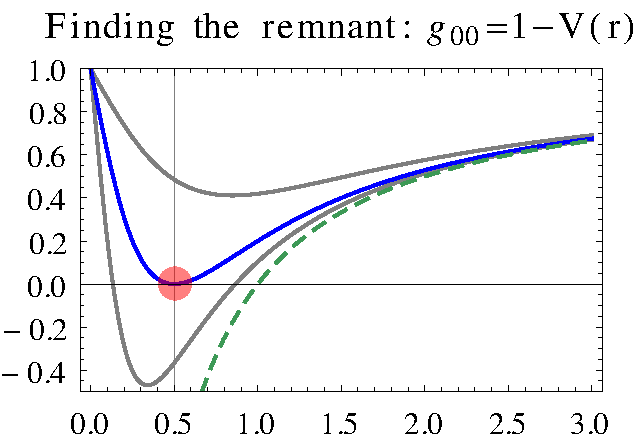
\includegraphics[width=10cm]{mathematica/remnant-plot.pdf}
\caption{Extremal Configuration in regularized Schwarzschild metrics. Since $g_{00}(r) \to 0$ at $r\in\{0,\infty\}$, there must be an extremal $r_0$. In the extremal configuration (blue), $r_0 = r_H$. There are also solutions with two $r_H$ and $r_0<0$ and no $r_H$, $r_0>0$. The dashed line is the Schwarzschild behaviour.}\label{fig:extremal}
\end{figure}

For our models (eq \ref{eq:start}), we can in general rewrite this set of equations in terms of $h(r)$. Especially, for finding the extremal value,

\begin{multline}
\partial_r V(r) = 0
   \Leftrightarrow  0 = \partial_r \frac{h(r)}{r^{n+1}}
   \Leftrightarrow  0 = -(n+1) \frac{h(r)}{r} + h'(r) \\
   \Leftrightarrow  0 = \left[L~h'(z)  -\frac{n+1}z~h(z)  \right]_{z=\frac{r_0} L}
\end{multline}

a substitution $z=r/L$ makes it easier to find a solution.

Finding the extremal radius $r_0$ (let $r_{0,\alpha}$ be for the self-regular model, $r_{0}$ for the holography model) is a bit of calculation. In the end, I got

\begin{align}
r_0 &= L ~\frac{1+n}{1-n} \label{eq:r0holo}\\
\highlight{ r_{0,\alpha} } &= \highlight{ \frac{L}{(1+n)^{1/\alpha}} } \label{eq:r0alpha}
\end{align}

\subsection{Extremal value for the holographic model $h(r) = \frac{r^2}{r^2 + L^2}$}
Equation \ref{eq:r0holo} tells us that there is {\it no extremum in higher dimensions}. At $n=0$ the result coincides with [NS2012], at $n>1$ all $r_0 < 0$. Actually this profile exhibits always a single horizon $r_H$ as soon as $n>1$. There is no more regularization for $n>1$ which can be read off the metric:

\begin{equation}
V(r) \propto \frac{1}{r^{n+1}} \frac{r^2}{r^2 + L^2}
\propto \frac{1}{r^{n-1}} \frac{1}{r^2 + L^2}
\end{equation}

As soon as $n>1$, there is a singularity at the origin. There is a special case in five dimensions ($n=1$). A naked black hole at origin can be made with $L=1$. etc.

\subsection{Self-Encoding for $h_\alpha(r)$}
The self regular solution looks like figure \ref{fig:extremal} in all dimensions. We can therefore always find a remnant and therefor fix $\alpha$ for any number of dimensions. Inserting $r_0$ to

\begin{equation}
1 \stackrel{!}{=}  V(r_0) 
   = \frac{2}{n+2} \frac{M(r_0)}{M_*^{n+2}} \frac{1}{\Omega_{n+2}}\frac{1}{r_0^{n+1}}  \frac{h_\alpha(r_0)}{1} \label{eqn:v1}
\end{equation}

After Calc6 (The surface issue), I think this equation needs some fixing. When $\frac{2\Omega_2}{\Omega_{n+2}}$ replaces the $\Omega$ fraction in equation \ref{eqn:v1}, in the $n\to 0$ limit this gives a $\frac{2\cdot 4\pi}{4\pi}$ which is needed to reproduce SMM correctly. Furthermore, let's remember that

\begin{equation}
M_P^2 = V_n M_*^{n+2},\quad V_n = (2\pi R_c)^n, \quad \frac{M_P=1/\sqrt{G}}{L_P=\sqrt{G}} = M_P^2 = \frac{1}{G},\quad \Rightarrow \frac{M_*}{L_*^{n+1}} = M_*^{n+2}
\end{equation}

Inserting $h_\alpha\left(L/(1+n)^{1/\alpha}\right)=\left(\frac{3+n}{2} \right)^{\frac{3+n}{\alpha}}$, I finally get

\begin{equation}
M(r_0) = \frac{1}{n+2} \left( \frac{3+n}{2} \right)^{\frac{3+n}{\alpha}} \left( \frac{r_0^{n+1}}{L_*^{n+1}} \right) \frac{\Omega_{n+2}}{\Omega_2} ~M_* \label{eqn:mr0}
\end{equation}

This looks very much like eq. 3 from [NS2012], expect the surface terms. The remnant's mass is equal to the reduced Planck mass if all coefficients get 1. This has multiple implications: We can determine $\alpha$ as well as identify $r_0 = L_*$, so the remnants radius is the reduced planck length. Eventually this means $L_P = (1+n)^{1/\alpha} L_*$. If I ignore the surface terms,

\begin{equation}
\alpha_0 = \frac{3+n}{\ln(2+n)} \ln \frac{3+n}{2}
\end{equation}

which reduces exactly to $\alpha_0 = \frac{3}{\ln 2} \ln \frac{3}{2}$ found by [NS2012] in $n=0$. Presumably they have to be taken into account, so

\begin{equation}
\highlight{\alpha_0 =  \frac{3+n}{\ln(2+n) - \ln \omega_n} \ln \frac{3+n}{2}}
,\quad \omega_n = \frac{\Omega_{n+2}}{\Omega_2} = \frac{\pi^{(n+3)/2}}{2\pi \Gamma\left( (n+3)/2 \right)}\quad\text{(Calc6, eq.5)} \label{eq:al0}
\end{equation}

This is fine, since $\omega_0=1$. I will use eq \ref{eq:al0} for further calculations.

\newpage
\begin{figure}[h]
\begin{center}
\begin{tabular}{ccccccccc}
\firsthline
 $n$ & 0 & 1 & 2 & 3 & 4 & 5 & 6 & 7 \\
   \hline
 $\alpha$  & 1.755 & 4.285 & 7.081 & 9.333 &
   10.642 & 11.128 & 11.098 & 10.805 \\
 $L_*$ & 1. & 0.851 & 0.856 & 0.862 & 0.86 &
   0.851 & 0.839 & 0.825 \\
 $M_*$ & 1. & 1.176 & 1.168 & 1.16 & 1.163 &
   1.175 & 1.192 & 1.212 \\
 $G_*$ & 1. & 0.724 & 0.733 & 0.743 & 0.739 &
   0.725 & 0.704 & 0.681 \\
   \hline
\end{tabular}
\end{center}
\caption{Self-encoding horizon radius $r_0=L_*$ and Remnant masses $M_* = 1/L_*$, in 4d Planck Units.}\label{table:L}
\end{figure}

\begin{figure}[h]
\center%
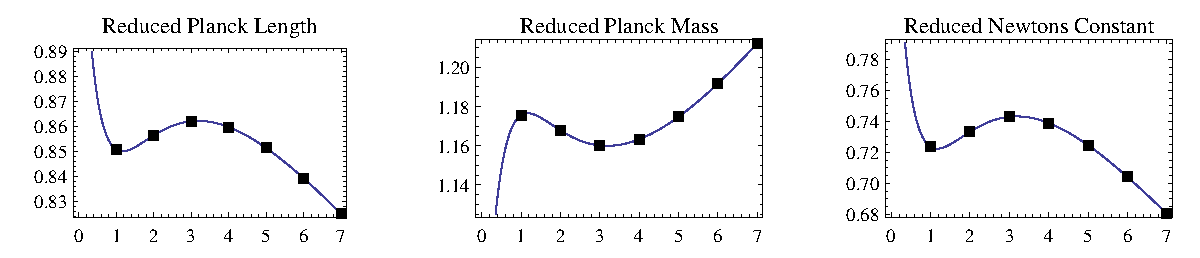
\includegraphics[width=\textwidth]{mathematica/table-graphs.pdf}
\caption{Table \ref{table:L} as plot, from left to right: $L_*(n)$, $M_*(n)=1/L_*$, $G_*(n)=L_*^2$}\label{fig:extremal}
\end{figure}

\section{Hawking Temperature}
Considering the $h_\alpha$ model with bigger masses $M>M_*$, the resulting Black Holes have multiple event horizons $r_H$. Solving $0=g_{00}$ gives (compare eqn \ref{eqn:v1}ff)

\begin{equation}
1 \stackrel{!}{=}  V(r_H) 
   = \frac{2}{n+2} \frac{M(r_H)}{M_*^{n+2}} \frac{1}{\Omega_{n+2}}\frac{1}{r_H^{n+1}}  \frac{h_\alpha(r_H)}{1} \label{eqn:h1}
\end{equation}

Eq \ref{eqn:h1} gives us the mass $M(r_H)$ of a BH with event horizon $r_H$ in the same was as eq \ref{eqn:mr0} told that for $M(r_0)$. Then I determine the Hawking Temperature $T_H = \frac{1}{4\pi} \left( \dd{g_{00}}r \right)_{r=r_H}$, plugging in $\alpha=\alpha_0$, $M=M(r_H)$. Let

\begin{align}
\label{hh1} V(r) &= A M(r) \frac{1}{r^{n+1}} h_\alpha(r) \\
\label{hh2} \Leftrightarrow M(r_H) &= \frac{r^{n+1}}{A ~h_\alpha(r)}
\quad\text{like in eq \ref{eqn:mr0}} \\
\label{hh3} \dd{g_{00}}r &= (n+1)\frac{M~A}{r^{n+2}} h_\alpha(r) - A~M\frac{h'_\alpha(r)}{r^{n+1}} \\
\label{hh4} \left.\dd{g_{00}}r\right|_{r=r_H} &= (n+1)\frac{1}{r_H} - \frac {h'_\alpha(r_H)}{h_\alpha(r_H)} \\
\label{hh5} &= \frac{1}{r_H} \left( 
 (n+1) - (n+3) \frac{1}{1+\left(\frac{r_H}{L}\right)^\alpha} \right) \\
\label{hh6} &= \frac{1}{L~z_H} \left( (n+1) - (n+3) \frac{1}{1+z_H^\alpha} \right)
\quad\text{with }z_H=r_H/L
\end{align}

Equations \ref{hh4}, \ref{hh5} and \ref{hh6} are wrong. Eq \ref{hh1}, \ref{hh2} and \ref{hh3} are correct.

\begin{figure}[h]
\center%
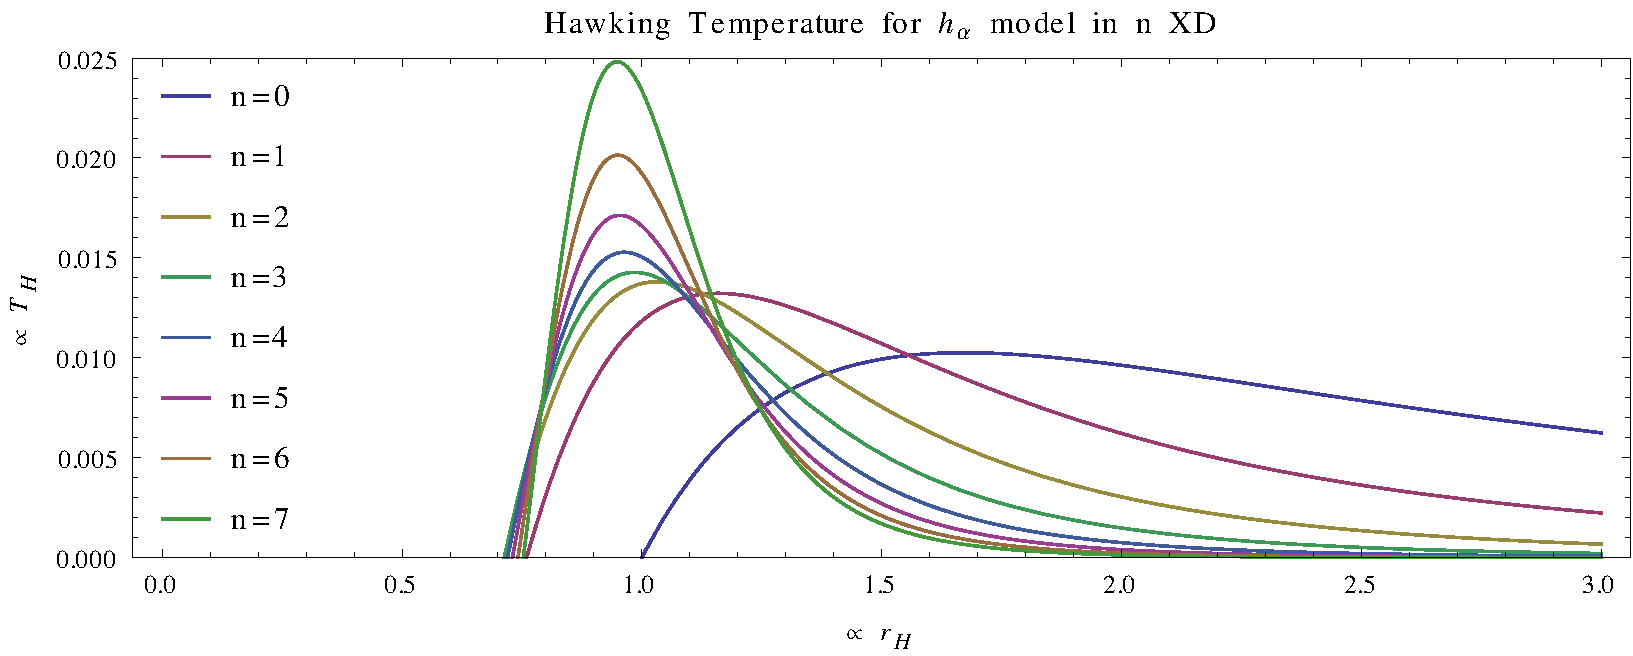
\includegraphics[width=\textwidth]{mathematica/Hawking-Temp-Plot.pdf}
\caption{Hawking temperature, plot of eqn. \ref{hh3} with $L=M=M_*=1$ and $\alpha=\alpha_0$. %\\ That is, on the y axis, $y=4\pi T_H / (M/M_*^{n+1})$
}\label{fig:th}
\end{figure}

%\newpage
The Hawking Temperature vanishes\footnote{I made a numeric check for $L=1$ like in figure \ref{fig:th}. I got a table (like figure \ref{table:L}) for the $r$ which solve the equation $T_H(r)=0$, the values match $r=L_*$ for all $n$.} at $r_0$, that is, $\highlight{T_H(r_{0,\alpha_0})=0}$. Again, this confirms the self-encoding property of $h_\alpha$.

\section{Heat capacity}
The Heat Capacaity $C$ is defined as $C=\partial U/\partial T_H$ with the internal energy $U=M$, so [NS 06.11.2013]

\begin{equation}
C = \frac{\partial M}{\partial T_H}
\end{equation}

I wonder how this works. In SMM ($G=1$), $T_H = 2M / r^2$, so $M = T_H r^2 / 2$ and $\partial M/\partial T_H = r^2 / 2$. This is not $C \propto -r^2$ as stated in [NS 06.11.2013]. Is it correct that

\begin{equation}
\pp MT = \left( \pp TM \right)^{-1} = \left( \frac{T}{M} \right)^{-1} \propto T^{-1}
\end{equation}

because is there is also the simple relationship $T_H = M ~f(r)$? This shows $-1/T_H$:

\begin{figure}[h]
\center%
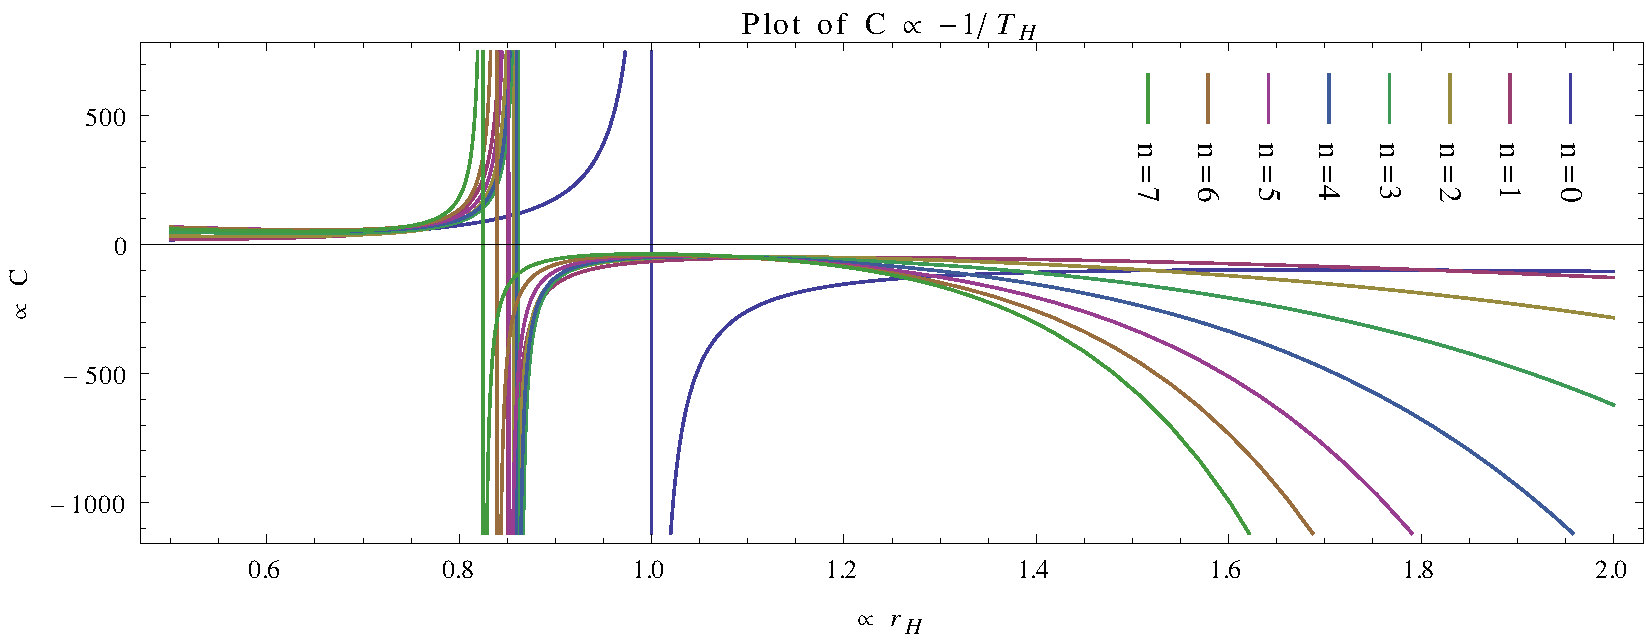
\includegraphics[width=0.8\textwidth]{mathematica/heat-capacity.pdf}
%\caption{blabla}
\end{figure}



\end{document}